\documentclass[a4paper,onecolumn,10pt]{book}

 

\usepackage{times}
\usepackage{listings}
\usepackage{graphicx}
\usepackage[colorlinks=true]{hyperref}
\usepackage[latin1]{inputenc}
\usepackage[T1]{fontenc}
\usepackage{mdwlist}
%\usepackage[english]{babel}

\newcommand{\jmethod}[1]{\texttt{\small #1()}}
\newcommand{\jclass}[1]{\texttt{\small #1}}
\newcommand{\JAVA}{\textsc{Java}}
\newcommand{\Sun}{Sun Microsystems}
\newcommand{\mswin}{Windows}
\newcommand{\unix}{\textsc{Unix}}
\newcommand{\file}[1]{\href{#1}{file:}}

 
\newcommand{\xmlswing}{\textsc{Xml4Swing}}
\newcommand{\tag}[1]{\textsf{<#1>}}
\newcommand{\attr}[1]{\texttt{\small \textbf{#1}}}
\newcommand{\classtag}{\tag{class}}
\newcommand{\nametag}{\tag{name}}
\newcommand{\implement}{\emph{\small \textsc{(to be implemented)}}}

\newcommand{\question}{\par\flushleft\textbf{Question:\ }}
\newcommand{\response}{\\\textbf{Answer:\ }}

\let\olditemize=\itemize
\def\itemize{
\olditemize
\setlength{\itemsep}{-1ex}
}



\title{\xmlswing}
\author{\small William R (\url{http://wrey.free.fr/})\\\textsc{SourceForge.org}}


% Choix du langage de l'affichage enrichi du listing
\lstset{language=java,%
    showstringspaces=false,%
    frame={trbl},%
    lineskip=-1pt,%
    extendedchars=true,%
    basicstyle=\footnotesize\ttfamily,%
    numbers=left,%
    stepnumber=5,%
    numberstyle=\tiny,%
    xleftmargin=2em,%
    }
\urlstyle{same}

 
\begin{document}
\maketitle

\tableofcontents
\sloppy

\chapter{Welcome}
\section{Abstract}
\xmlswing\ is a tool to create swing templates based on a
XML file. The developer provides a XML file and the software
will create a source code (not a compiled class) with all
the stuff necessary to have a graphic user interface in Swing.

The main difference with other tools proposed are:
\begin{itemize}
  \item Provides a JAVA source code.
  \item Integrates ``out-of-the-box'' features (look and
  		feel menu, etc.)
  \item Some helpful way to manage the AWT-Thread.
  \item Components organized on a HTML \verb|<table>| style (alignments,
  			grouping, etc.).
  \item Native SWING components extensions are possible.
\end{itemize}


\section{Using native interface}
Now, there are many providers giving you good solutions to create
your own GUI. The idea behind the \xmlswing{} is to give a way
for writing simple graphic interfaces very fast. Not only the
display itself but also programming a SWING application.


The program will help to create plain JAVA source code you have to
extend with your own class. You should NEVER use directly the code generated
by the program. Creating an GUI using the swing library is a natural
choice for creating basic things. If you want beautiful and more than
modern graphical interfaces, use JavaFX instead (but be careful, it is not 
part of the OpenJDK project and subject to licences). We just provide a
basic software with an open source code.

You simply have to provide all the things to put together in your GUI.
Only give names to components you want to control
(as a \verb|JTextField|). Menus can be generated quickly (and XML is
the best way to describe them): for each menu, you simply give the method
for processing the code behind.
 

About the licence: you can use this software for any purpose. The generated
classes can be distributed in binary mode or with the source code included. When
your development provides the \verb|.java| code source, it must be also
provide the \verb|.xml| file used to generate it (if possible in the
same directory or in the resource directory if you use Maven). This is typically non sense to distribute the source code
generated by this software but without the original XML file.

Note some of the functionalities described in this document
may be not yet implemented. Send me a request directly if needed.

\section{How it works}
You write an XML file containing the GUI interface you want. Normally, only
the graphical part is expressed in this file. Once the XML file is ready, you
run the software and it will generate a \JAVA\ code source in the
right directory (you can specify the directory in arguments). The class created
includes a \jmethod{main} method to test the graphical interface but you
have to create your own class based on the generated one to add the logic.
 

The generated class includes:
\begin{itemize}
  \item A \jmethod{main} method for test purposes.
  \item A \jmethod{initComponents} method for initializing the graphical objects.
\end{itemize}


That's quite simple. Do not try to understand the generated code, I can
just say: ``It works'' but the swing implementation is a confusion addition
of multiple things including menus, components, layouts and some other
stuff.

\section{My first application}

\subsection{Create the frame}
Usually, all the GUI applications run into a \jclass{JFrame} object.
It is the base of our XML file. Write the code of the figure \ref{fig:first-jframe}.
It will create a very simple frame but with all the stuff needed.

\begin{figure}[htb]
\begin{lstlisting}[language=XML]
<?xml version="1.0" encoding="ISO-8859-1"?>

<JFrame 
  title="First frame" 
  name="com.oxande.xmlswing.example.AbstractSampleFrame"
  coolsize="300,150"
  icon="./forward16.gif">
</JFrame>

\end{lstlisting}
\caption{The minimal application}\label{fig:first-jframe}
\end{figure}

Of course, in respect of object abstracting, you should not use
the frame like this. Please create the following code to support
the frame.

\begin{figure}[htb]
\begin{lstlisting}[language=java]

package com.oxande.xmlswing.example;

public class SampleFrame extends AbstractSampleFrame {
}

\end{lstlisting}
\caption{The minimal implementation}\label{fig:first-java}
\end{figure}

If you use the same package than the frame object, it is
quite easy to support the graphical part. Now, you have to configure 
the \xmlswing\ program to generate the code. Then you have to
run it as follow (we consider you are in the root of your Maven 
workspace, where is stored the \verb|pom.xml| file):


\small
\begin{verbatim}
java -cp xml4swing.jar
     -d . 
     ./src/main/resources/com/oxande/xmlswing/example/tutorial.xml
\end{verbatim}
\normalsize

Then to run the sample created, please run your code as follow
(do not forget to add the root of your classes to your class path):
\small
\begin{verbatim}
java -cp ./target/classes
     com.oxande.xmlswing.example.example.SampleFrame
\end{verbatim}
\normalsize

And, the first application is created and display something
similar to what you have in figure \ref{fig:tuto-1}. It is the
first but quickly (I suppose) created application.


\begin{figure}[htb]
\begin{center}
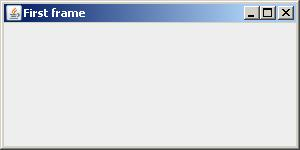
\includegraphics[width=0.5\linewidth]{tuto-1.jpg}
\end{center}
\caption{My first Application\label{fig:tuto-1}}
\end{figure}

Then, of course, it is very simple. Notice we didn't provide
the \verb|main| method for the application as we use the inherited one.
It is a good idea to create its own (figure \ref{fig:main}). You should
first instantiate the class. Then you initialize the components. In the last part, you set the frame to the visible mode.

\begin{figure}[htb]
\begin{lstlisting}[language=java]
public class SampleFrame extends AbstractSampleFrame {
   public static void main(String[] args)
   {
      SampleFrame appl = new SampleFrame();
      appl.initComponents();
      appl.setVisible(true);
   }
}
\end{lstlisting}
\caption{The main}\label{fig:main}
\end{figure}

Be careful, if you do this, when you close the window, the application
remains active. One way is to set the default close mode to
\verb|EXIT_ON_CLOSE|. But you have not to add new code: simply
add a tag to the XML file for the \emph{onClose} event. This event
is trigerred when the window is closed (i.e. the frame). See figure
\ref{fig:onclose} for the code added. It is quite simple, no? Now, your
application closes.

\begin{figure}[htb]
\begin{lstlisting}[language=XML]
<JFrame ...>
  <onClose>
     System.exit(0);
  </onClose>
</JFrame>
\end{lstlisting}
\caption{The minimal application}\label{fig:onclose}
\end{figure}

Another way to do is to use an attribute rather than the code
directly in the XML file. In this case, simply use the attribute
\verb|onClose="exit"| to give a method rather than the code.
You just have to implement this functionality by providing a
method as shown in figure \ref{fig:exitMethod}. Do not forget to
provide the method, if not the program will provide a default one
which throws an \verb|UnsupportedOperationException|.

\begin{figure}[htb]
\begin{lstlisting}[language=java]
public void exit(){
  System.exit(0);
}
\end{lstlisting}
\caption{The exit method}\label{fig:exitMethod}
\end{figure}

Now, you want to add a menu. Very simple, provide one as
cascaded menus in the XML file. Of course, we provide not
implemented ones. Each time, we provide a menu, the system
provide a default implementation showing a message saying it
is not implemented.

\begin{figure}[htb]
\begin{lstlisting}[language=XML]
<JFrame ...>
	<menubar>
    <menu>
      _File
			<item action="openFile">_Open File</item>
			<item>Close Fil_e</item>
			<separator />
			<item perform="exit">Exit</item>
		</menu>
		<menu>
			Help
			<lookandfeel />
    </menu>
  </menubar>
</JFrame>
\end{lstlisting}
\caption{The menu bar}\label{fig:menubar}
\end{figure}

The menu bar is simple. If you add \verb|action|s, you will
have something behing the menu. Note the ``\verb|_|'' (underscore)
sign to specify what letter will be underlined when the user
clicks on Alt button (for keyboard access). You should pay
attention to \verb|<separator/>| to simply create separators
and \verb|<lookandfeel/>| to have a complete menu to change
the look and feel of the application (evrything imported).

Note the \verb|action| attribute which points to the same \jmethod{exit}
method when the user close the window or select the \textit{Exit}
menu item.

\begin{figure}[htb]
\begin{center}
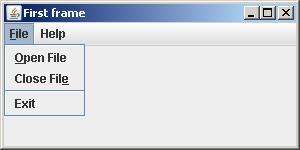
\includegraphics[width=0.5\linewidth]{tuto-2.jpg}
\end{center}
\caption{My first menu\label{fig:tuto-2}}
\end{figure}


\subsection{Add a status bar}

But, it is not the only the remarquable part. Now simply add the tag
\verb|<statusbar| \verb|id="statusBar"| \verb|property="statusMessage"| \verb|/>| and you have a status bar. Simply use the bean property
to set the message. You can write in your code \verb|setStatusMessage(msg)|
to change the status message. More than this, the change of the text is
made in the AWT-Thread because the text is changed by calling the
correct JAVA code to avoid an issue if you try to change the text
outside the AWT thread.

That's a king of magic. And the same is valid for the text objects
(\jclass{JTextArea}, \jclass{JTextField}, etc.) where the fact to set
the property permit to set it easily. But, please, don't look at the code
behind, it is a mess\ldots


\subsection{Add a toolbar}
As simple as for status bar, use the tag \verb|<toolbar>|
to add a toolbar (see section \ref{sec:JToolBar} for details).

\section{\label{sec:args}Arguments}
As for other JAVA programs, you must call the software using
the jar file (\verb|xml4swing.jar|) provided as follow:
\verb|java -cp xml4swing.jar| or add the jar file in the classpath
variable.

The complete command line becomes:
\verb|java -cp| \verb|xml4swing.jar| \verb|<arguments>| \verb|<templates>| where \verb|<arguments>| are the arguments shown below
and \verb|<templates>| the XML files which describe the different classes
to create. Using \verb|-| (the minus sign) as \verb|<templates>| will
use the standard input as XML file.


Please find below the arguments you can pass to \xmlswing:
\begin{itemize}
  \item \verb|-d <dir>|: the directory for sources. It is the base
  		of all your classes (basically \verb|${project_loc}/src/main/java|
  		if you use Maven.
  \item \verb|-V|: include the version. If set, a Javadoc tag
      \verb|@version| followed by the current date and time is added 
      in the source code of the class (do not use if you already have 
      a version control program as CVS or Subversion).
\end{itemize}



\chapter{Inside}

\section{The supported objects}
\subsection{\label{sec:Component}Component}
The root of all the supported graphical objects. Do not confuse with
the \jclass{JComponent} objects (which are the root components for
swing objects). There is no dedicated tag for an object: you should
always used a defined object.

Nevertheless, all the tags inherits of the following basic attributes:
\begin{itemize}
	\item \attr{minsize} the minimum size of the component expressed
		as a dimension (e.g. \verb|minsize="50,70"|). Not mandatory.
	\item \attr{maxsize} the minimum size of the component expressed
		as a dimension (e.g. \verb|minsize="100,130"|). Not mandatory.
	\item \attr{coolsize} the preferred size of the component expressed
		as a dimension (e.g. \verb|minsize="80,90"|). It refers
		to the \jmethod{setPreferredSize} method. Not mandatory.
	\item \attr{size} the size of the component expressed
		as a dimension (e.g. \verb|minsize="80,90"|). It refers
		to the \jmethod{setSize} method. Not mandatory.
	\item \attr{visible} you can hide the object by setting the
	  value to \verb|false|. Defaulted.
	\item \attr{cursor} set the cusor type. Can be one of the predefined
	  cursor (see section \ref{sec:cursors}). Not mandatory
\end{itemize}

\subsection{\label{sec:Container}Containers}
A container is (as its name says) a component created to store
graphical components (preferably \jclass{JComponent}s). A container
should have a layout and you can add several components in it.
On the other side, a graphical component is always a container! In fact,
I am not sure about the real use of the container as \xmlswing{}
use them internally but can not be created by the XML file itself
then you should nevr care about them.

\subsection{\label{sec:JComponent}Components}
A very generic class for all swing components (the famous
\jclass{JComponent}, the father of all the swing components). Inherits of the
\jclass{Container} (see section \ref{sec:Container}).

As for the \jclass{Component}, it is not possible to instantiate a
\jclass{JComponent}, you must use a more concrete objet. But a 
\jclass{JComponent} accepts the following attributes inherited by
all the other classes:
\begin{itemize}
	\item \attr{autoscrolls} can be set to \verb|true| to have automatic
		scrollbars if needed. Note this property can conflict
		with the \verb|hscroll| and \verb|vscroll| of the
		\jclass{JScrollPane} transparent implementation.
	\item \attr{background} set the background color. Any color is accepted.
	\item \attr{foreground} set the foreground color. Any color is accepted.
	\item \attr{doubleBuffered} is a boolean value to set a double buffering
		to the component. Should never set explicitly.
	\item \attr{enabled} is a boolean value to enable (\verb|true|) or
		disable (\verb|false|) a component.
	\item \attr{opaque} is a boolean value to call the method 
	  \jmethod{setOpaque} with the correct value. Should be never used.
	\item \attr{opaque} is a boolean value to call the method 
	  \jmethod{tooltip} all the components coming from swing can have
	  a tooltip. Simply set this attribute with a text for any component
	  to have a tooltip displayed when the mouse moves under the component.
\end{itemize}



 
\section{Buttons}
Buttons are used widely in GUI interfaces. The buttons are also
used to define menu items.

\subsection{\label{sec:AbstractButton}AbstractButton}
Inherits of \jclass{JComponent} (see section \ref{sec:JComponent}).
This component is used for generic buttons including
menu items (see section \ref{sec:JMenuItem}). If you set the
attribute \attr{property}, you will be able to know if the button
is selected or not (see figure \ref{fig:getsetbool}).
Note the \jclass{AbstractButton} is not linked to a concrete object
but the properties are used by the \tag{button}, \tag{radiobutton}
and \tag{checkbox} tags.

\begin{figure}[htb]
\begin{lstlisting}
public void setDebugMode( boolean debugMode ){
   button1.setSelected( debugMode );
}

public boolean getDebugMode(){
   return button1.getSelected();
}
\end{lstlisting}
\caption{Getter/setter for booleans}\label{fig:getsetbool}
\end{figure}

 
Abstract buttons have the following attributes:
\begin{itemize}
   \item \attr{selected} a boolean value specifying if the button
		is selected or not. useful for toggle buttons like radio
		buttons and check boxes.
   \item \attr{borderPainted} linked to the \jmethod{setBorderPainted}
		method. Can be set to \verb|true| or \verb|false|.
	 \item \attr{valign} set the vertical alignment of the button. Can be
	 \verb|center| (the default), \verb|top| or \verb|bottom|.
	 \item \attr{align} set the horizontal alignment of the button. Can be
	 \verb|right| (the default), \verb|left|, \verb|center|,
	 \verb|leading| or \verb|trailing|.
	 \item \attr{vtextalign} set the vertical alignment of the text.
	 \item \attr{htextalign} set the horizontal alignment of the text.
	 \item \attr{gap} set the icon gap. This is the number
	 of pixels between the icon and the text.
	 \item \attr{multiClickThreshold} value for modifying the threshold
	 between 2 cliks of the mouse. This value should be not modified as
	 it is linked to the normal behaviour of the GUI interface.
	 \item \attr{rollover} set to \verb|true| to activate the rollover.
\end{itemize}

\subsection{\label{sec:JButton}JButton}
A tag \tag{button} represents a normal button a user can
click (a \jclass{JButton}). The class inherits of the
\jclass{AbstractButton} described above.

The components has the following attributes:
\begin{itemize}
	\item \attr{default} set to \verb|true| to set the button
	as the default one. When the user press the enter key, the
	default button is selected.
	\item \attr{toggle} set to \verb|true|, the button is a
	toggle button (\jclass{JToogleButton}) rather than 
	an ordinary one\footnote{It is an hack in the XML notation
	as the tags are not bivalent for the other swing objects.}.
\end{itemize}

You must provide an attribute \attr{text} or the text directly
in the tag to set the text of the button. You can include
directly the mnemonic as specified in section \ref{sec:textcontents}.

A toggle button supports the \attr{property} attribute to set
and get directly the selected attribute of the button.

%   \item \verb|group| gives the group name where the button is.
%		You use groups for radio buttons where only one button
%		of the group is selected. The group name is exported as a
%		protected variable then the name must not conflict.

%   \item \verb|text| to set the text for this button. Note the text
%		can be given directly as the tag contents. The text can include
%		a mnemonic specifier (see section \ref{sec:textcontents}).

\subsection{\label{sec:JCheckBox}Check boxes}
Check boxes are buttons which can be selected or not. They inherits
of the properties of a \jclass{JButton}. The tag \tag{checkbox} must be
used.

You can also use the \tag{input} tag with the attribute \attr{type} equals
to \verb|checkbox| (this ensure a compatibility with HTML).

\subsection{\label{sec:JRadioButton}Radio buttons}
Radio buttons are buttons which can be selected or not. They inherits
of the properties of a \jclass{JButton}. 

The tag \tag{radiobutton} must be used. Note you can also use the 
synomnym \tag{radio} for the radio buttons. As for check boxes,
you can use the \tag{input} tag with the attribute \attr{type} equals
to \verb|radio| (this ensure a compatibility with HTML).

Radio buttons should be put in a group because the selection of
a radio button unselect the other radio buttons of the same group.
You just have to add the \attr{group} attribute with a group name
to include the radio button in a group.

\section{\label{sec:JTextComponent}Text components}
Inherits of \jclass{JComponent} (see section \ref{sec:JComponent}).

If you declare the attribute \verb|property|, you can use the
getter and setter property to set or get the text in the component. This
is a helper and a good solution to hide the object itself (an anonymous
object is de facto declared as \emph{private}). If you declare the
property as \verb|zipCode|, you will have 2 methods as you can see in
figure \ref{fig:getset}.


\begin{figure}[htb]
\begin{lstlisting}
public void setZipCode( String zipCode ){
   text1.setText( zipCode );
}

public String getZipCode(){
   return text1.getText().trim();
}
\end{lstlisting}
\caption{Getter and setter}\label{fig:getset}
\end{figure}


Please add a ``\verb|%|'' (percentage sign) after the variable name to
have a getter and a setter using an \jclass{int} type (rather than a
\jclass{String}).


\subsection{\label{sec:JPasswordField}Password fields}
The password field inherits of the \jclass{JTextField} (see section
\ref{sec:JTextField}).

It has the following attributes:
\begin{itemize}
  \item \verb|echo| the echo character to be displayed instead of
			the characters. It is a single character.
\end{itemize}

 
Note: the \verb|property| attribute can be used and you will be able
to get or to set the password as a normal text. If you use the component
directly, you must use the \jmethod{getPassword()} method to get
the password. See the javadocs for more information.

 
\subsection{\label{sec:JTextArea}Text areas}
The \tag{textarea} tag is declared using the \jclass{JtextArea} class and inherits the
\jclass{JTextComponent} (see section \ref{sec:JTextComponent}).
 
A text area is an area to input several lines of plain text. Supports the
\attr{hscroll} and \attr{vscroll} attributes.

\subsection{\label{sec:JTextField}Text fields}
The text field is declared using the \jclass{JtextField} class and inherits the
\jclass{JTextComponent} (see section \ref{sec:JTextComponent}).
 

\subsection{JSlider}
The \tag{slider} implements the \jclass{JSlider} class inherited from
the \jclass{JComponent} class.

The attributes are:
\begin{itemize}
	\item \attr{property} to have a getter and a setter for the value.
		The methods provide an \jclass{int} property. It is useful to
		get and set the value of the slider without manipulating it
		directly.
	\item \attr{orientation} can be \verb|horizonal| or
		\verb|vertical|.
  \item \attr{minimum} is the minimum value for the slider.
	\item \attr{maximum} is the maximum value for the slider.
  \item \attr{paintLabels} determines whether labels are
		painted on the slider (boolean).
  \item \attr{paintTicks} determines whether tick marks are
		painted on the slider (boolean).
  \item \attr{paintTrack} determines whether track is
		painted on the slider (boolean).
  \item \attr{snapToTicks} Specifying \verb|true| makes the
		knob (and the data value it represents) resolve to
		the closest tick mark next to where the user positioned
		the knob.
  \item \attr{majorTickSpacing} sets the major tick spacing
		(integer).
  \item \attr{minorTickSpacing} sets the minor tick spacing
		(integer).
  \item \attr{extend} sets the size of the range ``covered'' by the knob.
		Most look and feel implementations will change the
		value by this amount if the user clicks on either side
		of the knob. This method just forwards the new extent
		value to the model.
\end{itemize}

\section{\label{sec:JTable}Java tables}
The \jclass{JTable} class is useful to display your data.
You can display your table with the tag \tag{JTable} (do
not confuse with the tag \tag{table} used for formatting the
layouts).

Inside the tag, the attribute \attr{model} gives you the
opportunity to provide your own table class (must inherit
of the \jclass{TableModel} interface). You should give the
name of the model: you have to provide it through a initialization
\emph{before} initializing the GUI.

If you want to do some simple initialization without creating
your own table model, you can give the \tag{tr}, \tag{th} and
\tag{td} tags as you should do for a HTML table. Note there is
no alignment or other stuff: the data is displayed as simple
text in the table. This method is an helper to test your template
and not intended to be used in a production environment.

The figure \ref{fig:jtable} shows an example to display
a table table containing two files with some attributes.

\begin{figure}[htb]
\begin{lstlisting}[language=XML]
<JTable>
  <tr>
    <th>File Name</th>
    <th>Size</th>
    <th>Creation Date</th>
    <th>Modification Date</th>
  <tr>
  <tr>
    <td>xml4swing.properties</td>
    <td>1,5K</td>
    <td>18 Oct 2010</td>
    <td>7 Nov 2010</td>
  <tr>
  <tr>
    <td>Othello (Orson Wells)</td>
    <td>700Mo</td>
    <td>13 Oct 2003</td>
    <td>8 Jun 2005</td>
  <tr>
</JTable>
\end{lstlisting}
\caption{Example of JTable}\label{fig:jtable}
\end{figure}


 
\subsection{\label{sec:JApplet}Applets}
An applet (\tag{applet}) inherits of the \jclass{Container} class (section
\ref{sec:Container}).

An applet can contain a menu bar (as for a frame) and a main component
which is the \emph{content pane} as defined by the \JAVA{} API (see
method \jmethod{setContentPane}). Note a \jclass{JFrame} is a valid
container for an applet.

This component is very simple as it supports only the \verb|status|
attribute enabling to give the status of the applet. If you need an applet
with a complete support, you can add a \jclass{JFrame} (tag \tag{frame}) as
the main component of the applet.


\section{Special attributes}
\subsection{\label{sec:cursors}Cursors}
The attribute \attr{curosr} available for all components (including those
from the \jclass{java.awt.*} package) can have the following values:
\begin{itemize}
	\item \verb|crosshair| CROSSHAIR\_CURSOR
	\item \verb|default| DEFAULT\_CURSOR
	\item \verb|hand| HAND\_CURSOR
	\item \verb|move| MOVE\_CURSOR
	\item \verb|text| TEXT\_CURSOR
	\item \verb|wait| WAIT\_CURSOR
\end{itemize}

\subsection{Icons}
Some graphical components (especially buttons and menu items) accept icons.
Currently, an icon can be declared as a classic attribute. The icon is an
URL. You should always gives a icon which is inside your code or available
at a WEB address. You can not specifiy a file on the disk. To do so, you must
do this manually though you own class.

If you specify an property value containing a ``\verb|:|'' (semi colon), you
will load the icon directly. If you specifiy a path, the system will use the
\jmethod{getResource} method to load the icon.

\subsection{Names and References}
When you provide a \attr{id} attribute to a component, the component becames
visible for the class which extends this one. This is useful to access the
object and to manipulate it (buttons, menus, etc.) even if it is not nessary
in many cases if you do not change the normal behaviour.
 

Another interesting property is the \attr{reference} one. If a object has been
previously declared in the XML, you can resuse it by giving only the
\attr{reference} property. All other properties will be ignored.

\subsection{Color attributes}
Several attributes accepts to receive colors. The colors can be
given in two different ways.

The first easiest way is to give the RGB values in a hexadecimal
form prefixed by the sign ``\verb|#|''. This is strictly the same
notation than for HTML and CSS color parameters. For example, the color
red will be ``\verb|#ff0000|'', the blue is ``\verb|#0000ff|'' and so
on.

The second method works fine with several basic colors like white, red,
green, cyan, etc. You simply write the color you want to use (it is not
case sensitive). The color set you can give is the color set available
in JAVA (red, blue, cyan, red, orange, yellow, gray, black and white).

\subsection{Insets attributes}
Insets are used to give some margins. The term \emph{insets} refers to
the \jclass{Insets} class in JAVA. Basically, it is simply four values
to give the space (expressed in number of pixels) on the top border, the
left border, the right border and the bottom border.

You have to give the 4 values separated by commas (as for dimensions). For
example: ``\verb|2,6,8,3|'' will give you 2 pixels on top, 6 on the left,
8 on the bottom and 3 on the right.

To simplify, if you give only one value, this value applies to the 4 parts
(top, right, bottom and left). This is the easiest way to give the margins.
If you give 2 values, the first is affected to the top and the bottom and
the second one to the left and the right.


\subsection{Property attribute}
To set the value of a field (text field), you can use the \attr{property}
attribute. This avoid to use a object identifier and to use the 
\jmethod{setText}/\jmethod{getText} methods directly. Rather than this, use
the property attribute to define a getter and a setter you can use as bean
property.

The value is replicated in the object. But note the setter is used in
conjunction with \jmethod{SwingUtilities.invokeLater} to ensure the
system is not corrupted because you try to set the value from a thread which is
not the EDT thread (dedicated to swing management). Then the property is
set \emph{after}. If you do try to get the value just after set it, you can
have the old value (as the getter does not rely on the EDT thread management).

This is a good thing if you modify the text of the status bar through the
property rather than directly. In addition, you can expect better performances
if you often modify the value.
 
\subsection{\label{sec:Scrollable}Scrollable components}
Some components supports the \jclass{Scrollable} interface
(\jclass{JEditorPane}, \jclass{JFormattedTextField}, \jclass{JList},
\jclass{JPasswordField}, \jclass{JTable}, \jclass{JTextArea},
\jclass{JTextComponent}, \jclass{JTextField}, \jclass{JTextPane}, and
\jclass{JTree}). In this case you put the attributes \verb|vscroll|
and \verb|hscroll| to put the component in an anonymous \jclass{JScrollPane}.
 


The attributes can have the following values:
\begin{itemize}
	\item \verb|always| the scrollbar is always displayed.
  \item \verb|never| the scrollbar is never displayed.
  \item \verb|auto| the scrollbar is displayed only when needed.
\end{itemize}

The component is automatically encapsulated in a \jclass{JScrollPane}
if you give one of the property.


\subsection{\label{sec:textcontents}Text}
Normally the text of a button (including menu items) can have a mnemonic.
The text can be specified as an attribute \verb|text| or as a text contents
for the tag itself. It means \verb|<button text="OK" />| is equivalent to
\verb|<button>OK</button>|. If an attribute is given, it has a priority to
the contents of the tag.

 
You can specifiy a mnemonic for the text. It is very easy by preceding the
mnemonic by an underscore. For example \verb|<button>_OK</button>| will
permit to the user to type \verb|ALT|~+~\verb|O| to do the same than clicking
on the button.

Note the mnemonic is not case sensitive as we provide a key event rather than
a character. Only characters and digits should be used as mnemonics, other
characters will be ignored.


NOTES:
\begin{itemize}
  \item The ``\verb|_|'' (underscore character) has been choosen rather than the
		``\verb|&|'' (ampersand) because it is a special XML entity and needs to be
		escaped which is less easier when the XML is written without a dedicated
		editor\footnote{The ampersand character is used under the Windows SDK starting
		the beginning to create a menu keyboard short cut in the resources file}.
  \item Do not mix accelerators and mnemonics. A mnemonic can help to access the menu by
		typing the character when the menu is open. An accelerator is a combination of
		keys which gives the opportunity to have a direct access to the menu even if
		the menu is closed.
  \item The text is trimmed: the spaces at the beginning and the end of
    the text is deleted \emph{except} if given as an attribute.
\end{itemize}

 

\section{Menus}
Each item of a menu (\tag{item}, \tag{checkboxitem} or \tag{radioitem} can
have a \attr{action} task. The perform task should be mandatory
(at least for \tag{item}s): ff not
present, a \jclass{UsupportedOperationException} is thrown when the user clicks
the menu.

 
If \attr{action} is given as an attribute, it calls the specified method:
the method is declared as a \emph{protected} one and inherits the code specified
as ``Not implemented''. This is necessary to keep the class independant for
testing its behaviour (see section \ref{sec:testing}).
 

The specifications request a \jclass{ActionListener} class but the software will
provide the encapsulation and will call directly your method having no return
and no input parameter.

If you provide the action as a tag (\tag{action}), the text inside 
the tag is considered as
\JAVA\ code and will be implemented. This option is permitted to put simple logic
directly part of the GUI. That is a good solution to add a program exit or
some similar code. One limitation is you can not use instance variables (as
you can not provide any veriable in the GUI class).

 

\subsection{\label{sec:JMenuItem}Menu items}
The tags \tag{item}s gives you the capacity to add actions in your menu. Menu
items are based on abstract buttons (section \ref{sec:AbstractButton}). When
you define a menu item, it creates an associated \jclass{Action} interface:
this will help you for creating the toolbars for your application.

Note the text of the item can be provided as text in the tag itself or through
the \attr{text} attribute. The text can include the mnemonic information.

\subsection{\label{sec:JCheckBoxMenuItems}Check box items}
Very useful to set or unset an option. Same as menu \tag{item}s but do
not generate a ``Not implemented'' message when clicked.

\subsection{\label{sec:JRadioButtonMenuItems}Radio buttons items}
Very useful to set or unset an option in a group. Same as menu \tag{item}s but do
not generate a ``Not implemented'' message when clicked. You should
provide the \attr{group} attribute to group in the same group all the buttons.

 
\subsection{Look \& Feel}
I don't think it is the best idea, but you can push in any menu the
list of the available \emph{Look and Feels} available in the system
by adding the tag \tag{lookandfeel}. The entries are automatically
created and the selection is triggerred.

Note this should be done in the menu of the main frame to authorize
the system to refresh the GUI display. By default, selecting a Look 
and Feel option will automatically updates the GUI by refreshing the
frame container (found by calling the \jmethod{getRootPane} method).
You can override this behaviour by giving the object to refresh in
the \attr{refresh} attribute.

For you information, the look and feel is, by default, the ``Metal''
one. But, you can find the L\&F of your platform and update the
GUI accordingly. In this case, you must do this at the beginning of
your program because the L\&F must not be changed programmatically
after the \jmethod{init} method of the frame has been called.

\begin{figure}[htb]
\center
\begin{lstlisting}
public static void main( String[] args ){
   String name = UIManager.getSystemLookAndFeelClassName();
   UIManager.setLookAndFeel( name );
   // Put your code here...
}
\end{lstlisting}
\caption{How to configure the Look and feel.}
\label{fig:lookandfeel}
\end{figure}

\subsection{\label{sec:JToolBar}Tool bars}
You can define tool bars. Toolbars are made of \jclass{JComponents}. Then you
can encapsulate \emph{any} components. In addition, you can add separator (same
as for menus).


You can also add \tag{action} tags. An action tag is a simple way to say the
button in the toolbar is the same than the menu item (or any abstract button)
existing in a menu. Then you just add the reference to your menu item (of
course, you must give a name to your menu item first). In this case, the
toolbar inherits of the action linked to the menu item.

 
When you use actions (the prefered method), it is better to associate an icon
to your menu item.


In addition, the \tag{<toolbar>} tag has the following attributes:
\begin{itemize}
  \item \verb|floatable| boolean property to set to true for the user
		to move the tool bar.
  \item \verb|orientation| orientation for the toolbar. can be
		``horizontal'' or ``vertical''.
  \item \verb|rollover| sets the rollover state of this toolbar. If
		the rollover state is true then the border of the toolbar
		buttons will be drawn only when the mouse pointer hovers
		over them. The default value of this property is false.
  \item \verb|margins| set the margins. Must be 4 numbers seperated
		by commas.
  \item \verb|borderPainted| set the property to true if the border
		should be painted. The default value for this property is true.
\end{itemize}

 

\section{Panels and Layouts}
The main objective of this project is to remove the layout implementation.
This is why you don't hav to bother with the layouts. In the generated code,
you will find only 2 layout: the \jclass{FlowLayout} used to add components
in a simple way and the \jclass{GridBagLayout}.

\subsection{Table layout}
The table layout is based on the \jclass{GridBagLayout}. It is an
easier (and more HTML friendly) way to declare forms. You can simply
use the \tag{table} for the table, \tag{tr} for each row and \tag{td}
for the cells.

As for HTML tag, the \tag{td} can accepts the \verb|rowspan| and
\verb|colspan| attributes to span a cell on mutiple rows or cells.
You can use the \verb|align| attribute to align the component
(\verb|left|, \verb|right| or \verb|center|). For vertical
alignment, use the \verb|valign| attribute (possible values are:
\verb|top|, \verb|bottom| or \verb|middle|). You can put one
component only per cell (but can be a panel).


Note you can give a \verb|height| and \verb|width| parameter for
cell and this value will be transmitted to the component and will
change its preferred size accordingly \implement.


\subsection{\label{sec:JSplitPane}Splits}
In order to create a splitted view, you can use a \tag{split} tag.
This tag can split horizontally or vertically depending of your needs.
You can put in it any component (including container).
 

\begin{figure}[htb]
\begin{lstlisting}[language=XML]
<split orientation="horizontal">
   <pane>...<panel>
   <pane>...<panel>
<split>
\end{lstlisting}
\caption{Splitting panels}\label{fig:split}
\end{figure}

\section{High Level objects}
High level objects are object you can create. Currently,
you can creates \jclass{JFrame}s and \jclass{JDialog}s. Also,
menus can be create to help the context menus to enhance your
application.

\subsection{Frames}
A frame can be created with the \tag{JFrame} tag. Inside a 
\jclass{Jframe}, the primary layout is always a \jclass{BorderLayout}
where the top part is taken by the toolbar if you declare 
one\footnote{depending of your toolbar placement, the toolbar can go
to the left or right side}. The bottom part is for the status bar
(declared with the \tag{statusbar} tag).

The elements of your frame goes directly in the center of the panel
(the content panel). This behaviour sinplifies the development of
your interface. Of cours, you can create your own panels if needed.



\subsection{Dialog boxes}
Not yet implemented.

\section{\label{sec:testing}Unit testing}
In addition, the class generated includes a \verb|main| method to give you
the opportunity to test the generated code. The idea behind the test is to
open the frame (or the dialog) and to see the results.
 

The unit testing of a generated class disable the capability to the class to be
declared as an \emph{abstract} class. This is why all the methods are declared
\emph{protected} and provides a minimal behaviour: they throw a
\jclass{UnsupportedOperationException}. The developer is responsible to provide
the correct code in the extended class.
 
\chapter{Examples}
\section{File Explorer}
You know this under the name of \emph{Finder} if you are familiar with
the Apple environment. I named the program ``File Explorer'' as I coded under
a Windows box. Nevertheless, the code is not very complex.

The code is based on a simple frame. This frame contains 2 things: a tree
(\jclass{JTree}) on the left to display the directory tree and a plain list
(\jclass{JList}) for the list of the files found in the directory. The program
contains about 200 lines of code for the mechanism. You can add the same amount
of code for the GUI but generated automatically.

The main difficulty is to drive the tree: each time the user clicks on a 
directory, this directory and its content is loaded in memory\footnote{once
the directory loaded, changes on the disk are not visible on the screen, this
is a demonstration, not a real program.}. This part is the tricky part of the
code.

When you create the \jclass{Explorer}, you can use directly the 
\verb|pathTree| instance created by \xmlswing\ and \verb|fileList| also
created automatically. Then, you have just to implement the logic.

As you can see, the simple \tag{<statusbar>} creates a status bar you can 
access by its property name. The border is created to enhance the visibility
of the status bar. Also the font use is always a \emph{plain} one including
when the default look and feel is selected (the behaviour is to use a bold
font for labels). Use the \attr{property} method to set the text of
the status bar rather than relying directly to the button because of the
use of \jmethod{SwingUtilities.invokeLater} called at this time
rather than updating immediatly (if you come from a different thread than
the EDT one, you could have some issues).

One step is the creation and the management of buttons on the toolbar.
If you simply need actions also available in the menus, it is much more
simple and no code has to be written (except the XML declarations).


\chapter{Links}
Here some usefule links about the swing package and
other stuff related to graphic user interfaces.

\begin{itemize}
	\item \url{http://mbaron.ftp-developpez.com/javase/javavisu.pdf}
		a document about the classes \jclass{JTable} and \jclass{JTree}.
		Includes also a tutorial on the \jclass{JGraph} class.
	\item \url{http://gfx.developpez.com/tutoriel/java/swing/swing-threading/}
	  a cool document (in french).
	\item \url{http://java.sun.com/products/jlf/ed2/book/} A tutorial
	  about how to design dialogs and frames.
  \item
    \url{http://download.oracle.com/javase/tutorial/uiswing/layout/visual.html}
    It is a good place to learn about the layouts (even if this XML format
    has been conceived to avoid using the layouts directly).   
\end{itemize}

Here some concurrent projects:
\begin{itemize}
   \item \url{http://sourceforge.net/projects/jgb/} The project JDB on
   SourceForge.
   \item \url{http://sourceforge.net/projects/xml2swing/} Another
   project (but very simple, I think it has been cancelled).
   \item \url{http://netbeans.org/project_downloads/www/flashdemo/matisse.html}
   The Matisse project seems a good concurrent to this project giving
   you the capability to create the GUI with the mouse.
\end{itemize}


\section{Questions and Answers}
\question Is it possible to generate a class using only the
	\jclass{java.awt} package?
\response Basically, yes. But the package does not provide the
	XML tags for this. In addition, the XML focuses on the easy
	implementation of Swing components. Nevertheless, you can
	request the addition of the basic objects in this software.
	
\question Why generating a JAVA code source rather than providing
	a dynamic code?
\response This is the specificity of this tool: other good programs
	creates GUI interfaces on the fly. This is not the work of this
	software.
	
\question Can I create applets or dialog boxes?
\response This will be possible very soon. Currently, only the
	frames are available.

\end{document}

 
